% hoot.tex

% Author: Dustin Bachrach, Christopher Nunu, Dan Wallach, Matt Wright

% Revisions:  28 March 2011

\documentclass{acm_proc_article-sp}

\usepackage{mathptm}
\usepackage{times}
\usepackage{graphicx}

\begin{document}

\numberofauthors{4}

\author{
\alignauthor
	Dustin Bachrach\\
	\affaddr{Department of Computer Science}\\
	\affaddr{Rice University}\\
	\affaddr{Houston, Texas}\\
	\email{ahdustin@gmail.com}	
\alignauthor
 	Christopher Nunu\\
	\affaddr{Department of Computer Science}\\
	\affaddr{Rice University}\\
	\affaddr{Houston, Texas}\\
	\email{canunu@gmail.com}	
\alignauthor
	Dan Wallach\\
	\affaddr{Department of Computer Science}\\
	\affaddr{Rice University}\\
	\affaddr{Houston, Texas}\\
	\email{dwallach@rice.edu}\\
\and
\alignauthor
	Matt Wright\\
	\affaddr{Computer Science and Engineering}\\
	\affaddr{University of Texas at Arlington}\\
	\affaddr{Arlington, Texas}\\
	\email{mwright@cse.uta.edu}
}

\title{Hoot}
\date{May 6th, 2011}

\maketitle

\begin{abstract}

TODO:

\end{abstract}

\section{Introduction}

- Problem: Twitter like semantics w/ encrypted messages
	- Follow a Hash tag
	- Take hash tag and create something with crypto strength
	- Something derived from tags you can search on
	- But also deliberate collisions (cover traffic)
	
- Like to have thing that feels like twitter but anonymity properties:

- Twitter/Facebook relevant in Tunisia, (Social media playing big role in revolution across many countries. govt deliberately shut down)

- While we cannot keep them from filtering out service altogether,
want to have private communication in plain sight (not stenographic)

- Strong crypto usable by people whispering to each other in streets

- Only trusted channel is not electronic (spoken word), to exchange key.


- complimentary to Tor, solve problems Tor+Twitter does not

- What we are doing
-- Define a protocol for users to communicate over an insecure public network like twitter with message confidentiality and subscriber anonymity. 

- Punting on plain tag distribution

- Vocabulary

\section{Background}

1) History of government censorship, man in the middle
	- Tunisia code injection
	- Chinese firewall
	- Crypto keys for important services to iranian source (Komodo)
	- Person providing netwrok (even over ssl) might be evil

2) Tor
	- Trying to work against government censorship
	
- Group Crypto Keys
	
\section{Definitions}

- What is anonymous

- Cover traffic, k anonymity

- Privacy

- Define anonymity
--- Sender anonymity
--- Subscriber anonymity

- Basic Crypto:
	Message auth codes
	Hash Functions
	AES
	Vanilla crypto

\section{Design}

The Hoot protocol consists of a message header and a message body. The header contains the identifier, session key, digest key, and integrity digest. Messages are indirect in that they do not reference recipients. Anyone who knows the shared secret must be able to read the message, but should also be able to find the message easily. Rather than attempting to treat every message posted to Twitter as a potential group message, and thus decrypting the entire Twitter stream, the protocol places an identifier into every Hoot so a fellow group member can simply search for the identifier to see all potential messages. With a constant group identifier, readers can also publicly follow that identifier like any other Hash Tag on Twitter.

To create an identifier, we must find a short set of bits that are derivable from the shared secret, but give an attacker little information about the shared secret itself. Hash functions provide a great way to get a set of bits from a shared secret without divulging much information about the original shared secret. In our protocol, the shared secret is called a \textit{Plain Tag}, which is comparable to a Twitter Hash Tag. The result of hashing the Plain Tag with a given hash function, \textit{H}, is referred to as the \textit{Long Tag}. Thus,

\begin{equation}
	LongTag \leftarrow H(PlainTag)
\end{equation} 

The protocol could simply use the Long Tag as an identifier, but this choice leads to several problems. First, to uphold our design goal of being concise and to fit within Twitter's 140 character limit, it is infeasible to use the full output of a hash function. Secondly, strong hash functions do not produce many collisions. If a group is communicating in secret, not only do we want to protect the content of the communication, but we would like to conceal subscription to a particular group. For example, a rebellion group wishes to communicate over Twitter using Hoots, but it can be dangerous for a supporter of the rebellion to listen and subscribe to the identifier of the group. If, however, the identifier of the group can collide with the identifier of a popular Internet topic, like Charlie Sheen, group followers can shadow their rebellious activities 
with other innocent topics. 

To generate a collision, we need to shorten the long tag, generating a \textit{Short Tag}, which will induce more collisions. The shorter the Short Tag, the higher the collision rate will be and the less sure an observer can be of what topic a Hoot reader is listening to. With this greater anonymity comes more computational work, however. Since more group messages will now be belong to the same identifier, a follower must decrypt more messages to find relevant signal. Depending on the required degree of subscriber anonymity, more collisions might be worth the computational overhead. Also, even given a constant Short Tag length, a group can choose a tag that will collide with extremely popular tags to generate even more noise. Given a Long tag of byte-length \textit{N}, we produce a Short Tag by taking the first \textit{K} bytes of it:

\begin{equation}
	ShortTag \leftarrow LongTag_{[0:K]} : K < N
\end{equation}

The header also contains an set of encrypted keys, \textit{(Session Key, Digest Key)}. To combat replay attacks, the protocol uses a random session key to encrypt the plain text. This session key is then included in the set of keys in the header. The protocol ensures integrity the standard way by including an HMAC of the cipher text. The key to the HMAC function is randomly generated and is included in these set of keys: 

\begin{align}
	& SessionKey \leftarrow randomBytes() \\
	& Digest Key \leftarrow randomBytes()
\end{align}

To encrypt this set of keys, we exploit the entropy of the Long Tag. Since the identifier for a message is only the first \textit{K} bytes in the Long Tag, we can use the latter set of bytes elsewhere. By encrypting the keys with part of the Long Tag, a reader can easily know the key to decrypt with since it is simply the hash of the Plain Tag, and we also do not require knowledge of two different secrets. Thus, given an encryption function and corresponding key, \textit{$E_{key}$}, we have the encrypted keys as:

\begin{equation}
	KeyPair \leftarrow E_{LongTag_{[(K+1):N]}}(SessionKey.DigestKey)
\end{equation}

The body of the Hoot is the cypher text, \textit{C}, of a message, \textit{M}, encrypted with the Session Key:

\begin{equation}
	C \leftarrow E_{SessionKey}(M)
\end{equation}

The header also contains the integrity digest, \textit{D}, of the cypher text, using the Digest Key in the header. By including an integrity digest, the protocol allows for quick verification that a message is for a specific group without having to decrypt the message. It also verifies that the Hoot has not been tampered with. 

\begin{equation}
	D \leftarrow HMAC_{DigestKey}(C)
\end{equation}

Therefore, a complete Hoot appears as:

\begin{equation}
	Hoot \leftarrow ShortTag.KeyPair.D.C
\end{equation}

\section{Implementation}

In this section we describe an implementation of the Hoot protocol we create for our prototype.

\subsection{Generating a Hoot}

The Hoot protocol can be implemented in a variety of ways using different encryption and hashing algorithms. We created a Python prototype that fully implements the protocol.

A Long Tag is generated by running a SHA256 hash over the Plain Tag. The first 128 bits of the Long Tag are dedicated to identification. We then take the first m bytes of the Long Tag to get a Short Tag, where m is the desired Short Tag length.

The session key is 128 random bits, and the integrity key is 160 random bits. These random numbers are concatenated together and then encrypted using AES with the last 128 bits of the Long Tag as the key.

The plain text is encrypted using AES with the session key as the key. An integrity check is created by performing an HMAC-SHA1 of the cipher text and the integrity key as the key.

With all components created, a Hoot can be generated by printing out a \# symbol,  the short tag, a space, the encrypted keys, the HMAC digest, and the cipher text.

\subsection{Message Length}

Given our goal to conform to Twitter, the final output of a message must be under the 140 character limit. Another goal is to be concise and use as little overhead as possible for the entire encryption process. Twitter has a very broad definition of a character. It is not simply ASCII characters, but UTF-8 as well. Based on the encoding, we can squeeze the encryption into even fewer characters. However, this manipulation has issues since many clients do not conform to UTF-8, and there will be little gain if the plain text itself is written in UTF-8. Our prototype can generate Base64 encoded messages or Unicode messages.

Base64 encoding is simple, universal, yet yields longer message sizes. Given a short tag of length $m$ and a plain text message of length $n$, a Base64 encoded message has

\begin{equation}
	m + 20 * floor(\frac{n}{16}) + 118
\end{equation}

characters. Assuming a Short Tag of 2 characters, to fit a Base64 encoded message into 140 characters, the plain text message can be at most 31 characters.

A unicode message on the other hand can be much shorter. Given $m$ and $n$, a Unicode encoded message has

\begin{equation}
	m + 12 * floor(\frac{n}{16}) + 64
\end{equation}

characters. Assuming again a Short Tag of length 2, a Unicode encoded message can fit within 140 characters when the plain text is at most 111 characters. By using Unicode, the Hoot protocol only uses 29 characters of overhead and can handle reasonable length messages. Obviously, if longer messages are needed, multiple Hoots can be posted, but by having such a low overhead, we are getting 79\% utility out of the 140 characters.

\section{Experiments}

We performed the following experiments using our prototype to validate the protocol.

\subsection{Cover Traffic}

% \begin{figure}[hash-dist]
% \begin{center}
% 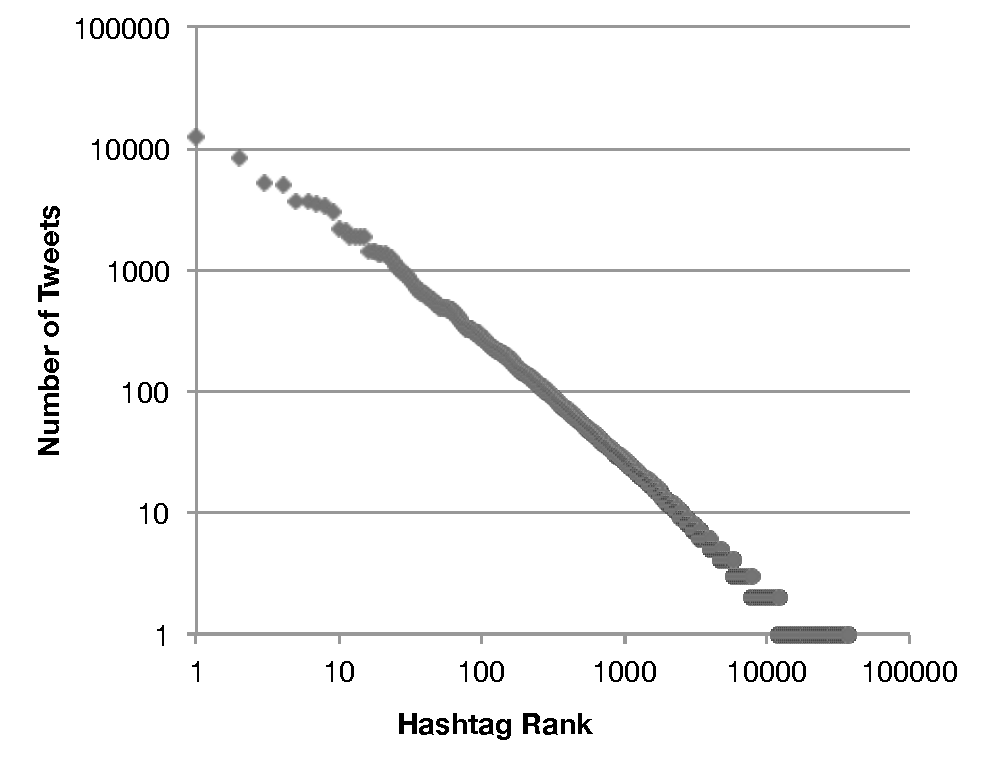
\includegraphics[scale=.25]{graphs/hash-tag-dist.pdf}
% \caption{2009 Twitter Hash Tag distribution on a log-log scale.}
% \end{center}
% \end{figure}

- Power log

- How long a short tag should be
- Collider
- Enough cover traffic?

- what that tells us about design parameters of solution

- Then we can conclude that we need this number of bits, etc
- Wrap up all experiments into What can our system do
<<<<<<< HEAD
	- Easy to collide or not to collide (Tune cover traffic)
	- Efficient computer message encryption
=======
	- Easy to collide or not to collide (Tune covertraffic)
>>>>>>> 43a047542b49d97052fd3efce939b1cda7954d58

\subsection{Performance}

In this experiment we wanted to see how well the encryption engine performed. In March 2011, Twitter stated that the site receives 140 million tweets per day or 1620 tweets per second on average (http://blog.twitter.com/2011/03/numbers.html). They also said that the maximum tweets per second ever was 6939. These numbers act as rough upper bounds to the number of Hoots per second the system would need to keep up with. In all likelihood, the number of encrypted messages posted would be drastically smaller than regular messages.

The following benchmarks were run on a 1.86GHz Intel Core 2 Duo, 4GB Ram, Macbook Air using Base64 encoding. 


\begin{table}
\caption{Average Hoots Per Second for Encryption and Decryption}
\begin{center}
    \begin{tabular}{ l  l }
	\hline
	Action & Average Hoots per second \\ \hline
	Encryption & 3614.531 \\
	Decryption & 15587.328 \\ \hline
    \end{tabular}
\end{center}
\end{table}

Given these numbers, a Twitter server could easily encrypt the entire Twitter feed as the messages were posted. To handle peak usage like the 6939 tweets per second Twitter observed, many optimizations could be made, the simplest being to add a couple computers to help with the load. Our experiment shows that the Hoot protocol does not have significant overhead during encryption or decryption, so it can be adopted with little engineering effort.

It is interesting to note that the decryption rate is important to a client, since a client will be searching tweets trying to identify and decrypt potential Hoots. A client may not trust Twitter to do the decryption since that involves sharing the Plain Tag with Twitter, so a client would decrypt the message on their machine. Almost every client will not have a datacenter of computers for decryption, but our  process can decrypt Hoots almost five times faster than it encrypts them. A client, even with limited computing power, can easily keep up with the Twitter feed.


\section{Discussion}

In this section, we discuss a variety of issues and future extensions of the Hoot design.

\subsection{Incremental Rollout}


1. Can you incrementally roll it out
	- Service provided by twitter or yourself
2. 140 character limit
	- Twitter doesn't have to go too far to have all the metadata for encryption
	
	- How hard is it for twitter to do this. 
	- Reference message fitting into 140 char using unicode
	- Reference peak hps, and how our system holds up

\subsection{Adoption}	

The next question to ask after we have shown that rolling out the Hoot service is feasible would be whether Twitter would actually implement such a feature. Based on the nature of Twitter, we believe that Twitter would not add a secure messaging framework like Hoot. Twitter as a company needs to know what people are talking about, so it can provide relevant advertisement. Adding the Hoot infrastructure to Twitter would prevent Twitter from knowing the content of the messages, and so we believe the Hoot service will never be adopted. However, this need not prevent individuals from using the Hoot protocol over Twitter. As long as Twitter faithfully delivers tweets, users are free to run the Hoot encryption on their own machines over their messages and then post the output to Twitter. In fact, this method is more secure in that a user only has to trust their machine. If Twitter is responsible for encrypting a message, nothing is stopping them from keeping a copy of the plain text message. Paranoid users will always want to encrypt messages themselves, so Twitter adopting the Hoot protocol is unnecessary.
		
\subsection{Usability}

As described in the Cover Traffic section, a group can deliberately collide with a popular tag by concatenating an easily rememberable string of text with random letters or numbers. As Miller noted in (The Magical Number Seven, Plus or Minus Two: Some Limits on Our Capacity for Processing Information), people can remember  
7 +/- 2 unique packets of data, so as long as these collisions can be generated with a suffix in that range a user is likely to be able to remember it. We could further improve rememberability by restricting suffix values to only digits, and then generate a suffix of 7 or 10 digits, emulating a phone number. The main requirement is that a group should be able to have a unique shared secret that can deliberately collide with other tags while still being easy to remember and more importantly easy to transfer. Since our proposal does not deal with key transfer, we assume our key communication is done through whisper channels and thus must be short and memorizable for simple transfer. We have found that a collision can be found with only appending 3-6 characters to a prefix, so deliberate collisions can both be found and transferred without much effort.
	
\subsection{Alternate Backends}

Even though our protocol was designed with Twitter in mind, it is extensible to other systems and platforms. The Hoot protocol describes a secure way to transfer short messages (with short encryption overhead) across a publicly available network completely openly. Twitter is a great example of this environment but not the only one. Hoot could interact, for example, with a Distributed Hash Table system (DHT) like CHORD or Pastry. Importantly, Hoot can interface with both centralized systems like Twitter or Buzz or decentralized systems. As long as the platform's content is publicly searchable, the Hoot protocol allows secure transmission to anonymous group followers.

\section{Conclusions}

TODO:

\bibliographystyle{abbrv}
\bibliography{hoot–bib}

\balancecolumns{}

\end{document}
